\documentclass[table]{beamer}

% Modèle proposé par Aurélie Boisbunon

% ATTENTION : IL FAUT EXECUTER LE CODE 2 FOIS POUR QUE LES IMAGES
% SOIENT AU BON ENDROIT

% Theme du poster
\usetheme{posterLITIS2}
%\usetheme{posterLITIS}

% Mise en page poster
\usepackage[orientation=portrait,size=a1 ,scale=1.2]{beamerposter} 


\usepackage[english]{babel}
\usepackage[utf8]{inputenc}
\usepackage{times} % Police du texte
\usepackage{amsmath,amsthm, amssymb, latexsym} % Packages pour
% formules maths
\usepackage{dsfont} % Package pour l'indicatrice

% Package et librairies pour dessins et figures : package 
\usepackage{pgf,tikz} 
\usetikzlibrary{calc,trees,positioning,arrows,chains,shapes.geometric,%
  decorations.pathreplacing,decorations.pathmorphing,shapes,%
  matrix,shapes.symbols,shapes.arrows}

% Pour surligner la ligne des tableaux
\definecolor{Mygrey}{gray}{0.8} 

% Couleur des sous-titres dans les cadres et du texte en vert
\newcommand{\soustitre}[1]{\vspace{5pt}{\small\textbf{\textcolor{bleuL}{#1}}}} % 
\newcommand{\exemple}[1]{\textcolor{vertL!92!black}{#1}} % 

\usepackage{multicol} %Pour la bibliographie sur 2 colonnes nottament
% Si on veut une image de fond
% \setbeamertemplate{background canvas} 
% { 
% \begin{tikzpicture}
%   \node[inner sep=0pt,xshift=20cm]  at (current page.center)
%   {
\includegraphics[width=.5\paperwidth]{LITIS_fond.png}};
% \end{tikzpicture} 
% } 

%   ******************************************************************************************
%   Definition des elements du graphe tikz
\tikzset{
  >=stealth',
  punktchain/.style={
    ellipse, 
    draw=rougeF!80, thick,
    top color=red!10,              % a shading that is white at the top...
    bottom color=rougeF!70,
    text width=4.3em, 
    minimum height=2em, 
    text centered, 
    on chain},
  line/.style={draw, ultra thick, <-},
  every join/.style={->, ultra thick ,shorten <=2pt,
    shorten >=2pt,},
}

% *******************************************************************************************
% EN-TETE ET PIED DE PAGE
% *******************************************************************************************

% Chemin pour repertoire d'images
\graphicspath{{imgs/}}

% Titre, auteurs, institut, date
\title{Affectation \ des \ opérations \ de \ déplacements \ de \ conteneurs : \ approche \ par \ colonies \ de \ fourmis}
\author[Lesauvage et al.]{Gaëtan Lesauvage, Frédéric Guinand, Stefan Balev}
\institute[LITIS]{Université du Havre}
% \date{Dec. 16th, 2011}

% Logos 
\newcommand{\logolitis}{logo_litis_bleu_transp.png}
\newcommand{\logoinstitut}{logo_univ_lehavre.png}
%\newcommand{\logolaboratoire}{logo_univ_lehavre.png}

% Pied de page avec adresse site Litis et adresses mail des auteurs
\newcommand{\foottextleft}{http://www.litislab.eu} % texte a gauche
\newcommand{\foottextright}{ gaetan.lesauvage@litislab.fr  } % texte a droite

% *******************************************************************************************
% CONTENT
% *******************************************************************************************

\begin{document}
\begin{frame}{} 
\footnotesize
  \begin{columns}
    \begin{column}{0.80\linewidth}
      \begin{block}{Abstract}
	
	\begin{itemize} 
	  \item Déterminer les listes ordonnées de déplacements de conteneurs, appelés \exemple{missions}, pour chaque \exemple{chariot cavalier}, afin de minimiser le temps de dépassement des fenêtres temporelles ainsi que la distance totale parcourue
	  \item Problème des \alert{multiples} voyageurs de commerce avec fenêtres de temps (\textit{M-TSP-TW})
	  \item Prise en compte de la \exemple{dynamique} : arrivée de nouvelles missions, modification des contraintes, etc
	  \item Résolution par \textcolor{vertL}{colonie de fourmis}
        \end{itemize}
      \end{block}
    \end{column}
  \end{columns}

  % *****************************************************************************************
  \vfill	
  \begin{columns}
    \begin{column}{.945\paperwidth}
      \begin{block}{Contexte~: terminal portuaire à conteneurs}
        \begin{columns}[c]
	  \begin{column}{.45\linewidth}
	    \soustitre{Transfert de conteneurs entre 3 zones~: }
          \end{column}
          \begin{column}{.50\linewidth}
            \soustitre{Chariots Cavaliers~:}
          \end{column}
          \end{columns}
          \vspace{-20pt}
	\begin{columns}[t]
	  \begin{column}{.45\linewidth}
	    \begin{figure}[h]
		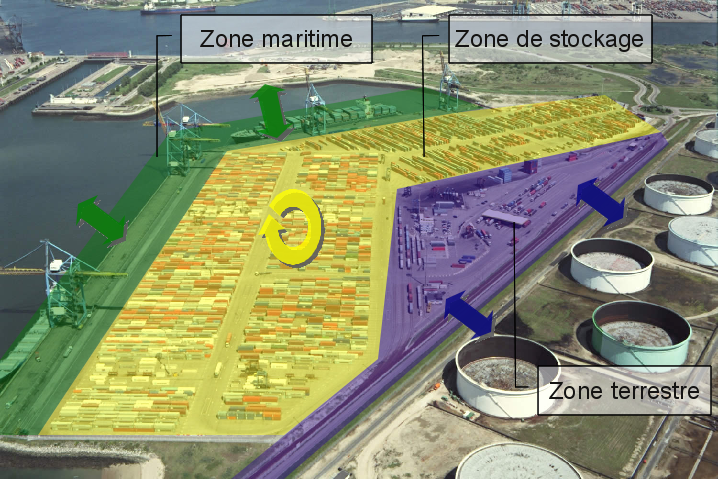
\includegraphics[width =0.6\linewidth]{3zonesDuTN}
	      \end{figure}
	   \end{column}
	   \begin{column}{.50\linewidth}
	      \begin{columns}[t]
	      \begin{column}{0.62\linewidth}
		\begin{itemize}
		  \item Prise de conteneurs par le dessus
		  \item Enjambent les travées
		  \item Capables de (dé)charger directement des camions
		  \item Stationnent au dépôt lorsqu'ils sont inutilisés
		  \item Mission : déplacer un conteneur dans le terminal
		  \item 2 phases : 
		  \begin{list}{-}{\leftmargin=2em}
		    \item collecte (Pickup)
		    \item livraison (Delivery)
		  \end{list}
		\end{itemize}
	      \end{column}
	      \begin{column}{0.35\linewidth}
		\begin{figure}[h]
	          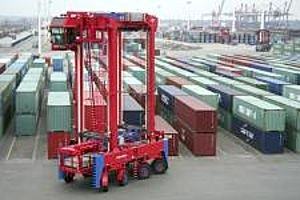
\includegraphics[width =\linewidth]{chariot_cavalier}
		\end{figure}
	      \end{column}
	      \end{columns}
          \end{column}
          \end{columns}
      \end{block}
    \end{column}
  \end{columns}

  % *****************************************************************************************
  \vfill
  \begin{columns}[t]
    \begin{column}{.945\paperwidth}
      \begin{block}{Modélisation}
      \vspace{-20pt}
	\begin{tabular}{p{0.55\linewidth} p{0.03\linewidth} p{0.4\linewidth}}
	  \soustitre{Multiple-Traveling Salesman Problem with Time Windows}
	  \begin{itemize}
	    \item Généralisation du problème classique de voyageur de commerce pour \alert{$m$} voyageurs \cite{Bektas2004}
	    \item Chacune des \alert{$n$} villes doit être visitée 1 fois par un des voyageurs
	    \item Chaque voyageur débute et termine sa tournée au dépôt
	  \end{itemize}
	  \begin{itemize}
	    \item Soit $G = (V,A,w)$ le graphe orienté complet composé des $n$ villes à visiter et de la fonction $w_k$ de pondération des arcs, dépendante du voyageur $k$.\\
	    \item Soit $T_v = \{T_v^{MIN} , T_v^{MAX}\}$ la fenêtre de temps associée à la ville $v$
	    \item Objectif : minimiser la durée de dépassement des fenêtres de temps ainsi que la distance totale parcourue~:
	    \begin{list}{-}{\leftmargin=2em}
	      \item Dominance de Pareto
	      \item Priorisation
	      \item Linéarisation : dépassement$\cdot F_1 + $distance$\cdot F_2$
	    \end{list}
	  \end{itemize}
	  &  \vspace{150pt} {  \LARGE $\Rightarrow$ } & 
	  \soustitre{Application au terminal à conteneurs}
	  \vspace{65pt}
	  \begin{itemize}
	    \item \alert{$m$} chariots cavaliers
	    \item \alert{$n$} missions
	    \item $w_k(i,j) = $durée$_{k}(i,j)+$durée$_{k}(j,j)$
	    \item \textcolor{vertL}{dynamique et incertitude~:}
	    \begin{list}{-}{\leftmargin=2em}
	      \item nouvelles missions
	      \item retards
	      \item pannes
	      \item $\cdots$
	    \end{list}
	  \end{itemize}
	\end{tabular}

      \end{block}
    \end{column}  
  \end{columns}
    % ****************************************************************************************
    
  \vfill
  \begin{columns}[t]
    \begin{column}{.945\paperwidth}
      \begin{block}{Méthode de résolution : approche par colonies de fourmis}
        \begin{multicols}{2}
        \begin{itemize}
        \item Modèle basé sur l'$Ant$-$System$ de Dorigo et al. \cite{Dorigo1992}
        \item $m$ fourmis, chacune avec sa propre phéromone
        \item Une fourmi peut coloniser un nœud du graphe s'il n'a pas été déjà colonisé par une des fourmis dans le tour courant
        \item La construction d'un tour consiste à choisir aléatoirement une fourmi parmi les $m$ disponibles afin qu'elle colonise un sommet (eq. 2), tant que tous les sommets n'ont pas été visités
        \item Lorsque tous les sommets ont été colonisés, le tour est évalué et si le score est meilleur que le record courant~:
	     \begin{list}{-}{\leftmargin=2em}
	      \item les fourmis déposent de la phéromone sur les arcs de leur chemin (eq. 1)
	      \item le record est mis à jour
	     \end{list}
	\item La solution au problème sera le meilleur tour $t$ parmi les $T$ tours construits
	\item Règle de dépôt de phéromone~:
	\begin{tabular}{p{.9\linewidth} p{.1\linewidth}}
	      \centering $\tau_{ij}=(1-\rho) \cdot \tau_{ij} + \rho \cdot \Delta\tau_{ij}$ & (1)
	\end{tabular}
	\begin{equation*}
 	  \text{Avec } \Delta\tau_{ij}=
 	  \begin{cases}
 	    1/L^* & \text{si } (i,j)\in \text{meilleur chemin global}\\
 	    0 & \text{sinon}
 	  \end{cases}
 	\end{equation*}
	\item Règle de transition proportionnelle~:
	\begin{tabular}{p{.9\linewidth} p{.1\linewidth}}
	      \centering $p^{m}_{i j} = \frac{\left({\tau^{m}_{i j}}\right)^{\alpha} \cdot
	      \left({\eta^{m}_{i j}} \right)^{\beta} \cdot 
	      \left ( \frac{\tau^{m}_{i j}}{\sum \limits_{l=1}^{M}{\tau^{l}_{i j}}} \right) ^\gamma}
	      {\sum \limits_{k \in V_{nonvisites}}{\left({\tau^{m}_{i k}}\right)^{\alpha} \cdot \left({\eta^{c}_{i k}}\right)^{\beta} \cdot \left( \frac{\tau^{m}_{i k}}{\sum \limits_{l=1}^{M}{\tau_{i k}^{l}}} \right) ^\gamma}}$ & (2)
	\end{tabular}
        Avec~: 
	\begin{list}{-}{\leftmargin=2em}
	  \item $\tau^{m}_{i j}$ : niveau de phéromone de la fourmi $m$ sur l'arc $(i,j)$
	  \item $\eta^{m}_{i j} =  \frac{1}{t^{m}(d_{i j})\cdot F_1 + l^{m}_{i j}\cdot F_2 + e^{m}_{i j}*F_3}$
	  \item $t^m(d_{i j})$~: temps de parcours de la distance entre les villes $i$ et $j$ par la fourmi $m$.
	  \item $l^m_{i j}$~: retard (lateness) de la fourmi $m$ à l'arrivée à $j$ en venant de la ville $i$ (dépend de la date de départ de la ville $i$).
	  \item $e^m_{i j}$~: temps d'attente (earliness) de la fourmi $m$ avant de pouvoir visiter la ville $j$ en venant de $i$ (dépend de la date de départ de la ville $i$).
	\end{list} 
      \end{itemize}
    \end{multicols}
    \end{block}
    \end{column}  
  \end{columns}

  % *******************************************************************************************
  \vfill
  \begin{columns}
    \begin{column}{.945\paperwidth}
      \begin{exampleblock}{Résultats préliminaires}
	\begin{center}
	 Simulations réalisées avec D$^2$CTS \cite{Lesauvage2011}. Paramètres : $F_1=1$ , $F_2=5$ , $F_3=10$ , $\alpha=1$ , $\beta=1$ , $\gamma=1$ , $\rho=0.1$ , $it_{MAX}=10^6$
	\end{center}
	\begin{center}
	  \begin{tabular}{p{0.4\linewidth} p{0.4\linewidth}}
	   
            \begin{table}[!h]
              \footnotesize
              \label{tab:n10m2results}
              \begin{tabular}{|c|c|c|c|}
               \hline
               \multicolumn{4}{|c|}{$m=2$} \tabularnewline
               \hline
               Problem & Score (\textbf{optimal}) & Itérations & Temps (Branch \& Bound)\tabularnewline
               \hline
               $P_1$ & \textbf{5832} (5832)& 15150 & 1.43s (15.83s)\tabularnewline
               $P_2$ & \textbf{4699} (4699)& 8541 & 0.62s (7.23s)\tabularnewline
               $P_3$ & \textbf{4294} (4294)& 206869 & 8.55s (6.71s)\tabularnewline
               \hline
               \end{tabular}
            \end{table}
            &
            \begin{table}[!h]
              \label{tab:n10m3results}
              \begin{tabular}{|c|c|c|c|}
               \hline
               \multicolumn{4}{|c|}{$m=3$} \tabularnewline
               \hline
               Problem & Score (\textbf{optimal}) & Itérations & Temps (Branch \& Bound)\tabularnewline
               \hline
               $P_1$ & \textbf{2742} (2742)& 404550 	& 19.59s (12m04s)\tabularnewline
               $P_2$ & 2830 (2827)& 542903 	& 27.22s (9m46s)\tabularnewline
               $P_3$ & 3106 (3103)& 227260 & 10.27s (12m39s)\tabularnewline
               \hline
              \end{tabular}
            \end{table}
           
        \end{tabular}\\
	 \textcolor{bleuL}{Table~:} Résultats pour 3 problèmes de taille $n=10$
	 
         
         \end{center}
      \end{exampleblock}
    \end{column}
  \end{columns}
  % *******************************************************************************************
  \vfill
  \begin{columns}
  % BIBLIO
    \begin{column}{.945\paperwidth}
      \textbf{Réferences}
      \vspace{-20pt}
      {\scriptsize
        \bibliography{biblio_poster}
        \bibliographystyle{nar}
        \begin{multicols}{2}
        \begin{thebibliography}{10}	
	  \bibitem[Dor92]{Dorigo1992}
	  M.~Dorigo.
	  \newblock {\em {Optimization, Learning and Natural Algorithms}}.
	  \newblock PhD thesis, Politecnico di Milano, Italy, 1992.
	  
	  \bibitem[Bek06]{Bektas2004}
	  T.~Bektas.
	  \newblock {The multiple traveling salesman problem: an overview of formulations
	    and solution procedures}.
	  \newblock {\em Omega}, 34(3):209--219, jun 2006.
	  
	  \bibitem[Les2011]{Lesauvage2011}
	  Ga{\"e}tan Lesauvage, Stefan Balev, and Fr{\'e}d{\'e}ric Guinand.
	  \newblock {D$^{2}$CTS} : A dynamic and distributed container terminal
	  simulator.
	  \newblock In {\em HMS 2011 : The $13^{rd}$ International Conference on Harbor,
	  Maritime {\&} Multimodal Logistics Modelling and Simulation}, September 2011.
	  
	\end{thebibliography}
	\end{multicols}
      }
    \end{column}
  \end{columns}

\end{frame}
\end{document}



%%%%%%%%%%%%%%%%%%%%%%%%%%%%%%%%%%%%%%%%%%%%%%%%%%%%%%%%%%%%%% 

%%% Local Variables: 
%%% mode: latex
%%% TeX-PDF-mode: t
%%% End:
